\clearpage{\pagestyle{empty}\cleardoublepage}
\chapter{Validazione}

\section{Metodologia di test}

La metodologia di test adottata è quella del \emph{unit testing}, per poi arrivare al test dell'intero sistema.

Prima di tutto sono stati verificati i requisiti funzionali, dopodiché si è passati a test atti a mettere sotto stress il singolo componente, al fine di valutare le performance ottenibili e quindi migliorarle.

Nel fare questo, sono comunque stati svolti dei test di regressione, in modo che i cambiamenti apportati garantissero ancora la piena funzionalità del componente, e quindi del sistema.

\section{Test sulla flowHashTable e libreria nDPI}

Per quanto riguarda questi due componenti, poiché strettamente connessi, si è scelto di testarli assieme attraverso un file specifico (\emph{test\_hash\_pcap}).

Il test consiste nell'aggiungere ad una flowHashTable tutti i pacchetti IPv4 con protocollo di trasporto TCP e UDP contenuti in un file PCAP specificato da riga di comando, per analizzarli tramite la libreria nDPI, come se si trattasse di normale esecuzione.

Naturalmente, il primo aspetto rilevato è quello di funzionalità, cioè se effettivamente i vari flussi venivano salvati correttamente. Sono quindi stati usati file PCAP di piccole dimensione (anche solo una decina di pacchetti per averne il massimo controllo), con una stampa delle informazioni contenute nella tabella hash al fine di rilevare la congruenza tra dati immessi e dati immagazzinati. In questo caso la libreria nDPI è stata solo usata al fine di riconoscere i protocolli applicativi, facendo quindi una stampa di quelli trovati.

Dopo aver constato questo, si è proceduto con test più stressanti nei confronti della struttura dati e della libreria, con operazioni su file PCAP di oltre 250 mila pacchetti al fine di rilevarne le prestazioni. A questo scopo sono stati rilevati i cicli di clock consumati (facendo la differenza tra i cicli ritornati dalla chiamata alla funzione \emph{rdtsc} effettuata prima e dopo) per fare un'operazione di inserimento nella tabella hash e un'operazione di riconoscimento del protocollo applicativo.

Avendo questo \textit{$\Delta$ cicli di clock} per ogni operazione, si sono potuti ricavare i principali indici statistici per effettuare delle analisi qualitative. In particolare si è calcolato minimo e massimo, media, deviazione standard. Inoltre si è cercato di stabilire la distribuzione in base a fasce di cicli di clock ritenute ottime.

Per quanto riguarda la libreria nDPI si è ottenuto che in media ci vogliono 870 cicli di clock per tentare di riconoscere il protocollo applicativo con una deviazione piuttosto alta (intorno ai 2700 cicli). Si è però riscontrato come circa l'83\% dei pacchetti venga processato con meno di 1000 cicli, l'8\% con 1000-1500, e altrettanti con oltre 1500.

Sono risultati di tutto rispetto se si pensa all'analisi approfondita che bisogna compiere su ogni pacchetto, ma sicuramente ancora migliorabili.

La tabella hash invece è stata la struttura dati in cui si poteva avere molta scelta per quanto riguarda la realizzazione. Seguendo la realizzazione standard e più semplice, i risultati non erano molto entusiasmanti (si parla di una media intorno ai 1500 cicli di clock, con una deviazione oltre i 3000).

Ci si è quindi mossi verso l'implementazione mediante i principi detti nell'apposita sezione \ref{impl-fht} del capitolo sull'Implementazione, ottenendo davvero ottimi risultati.

\clearpage
L'operazione di aggiunta delle informazioni di un nuovo pacchetto nell'hash table (che ricordiamo essere realizzata con ricerca del flusso relativo, eventuale riuso di una vecchia struttura o creazione di una nuova) costa mediamente 330 cicli di clock, con una deviazione intorno ai 1200 cicli. Potrebbe sembrare un pessimo valore, ma l'analisi per fasce ha evidenziato come circa il 95\% dei pacchetti venga aggiunto con meno di 400 cicli, il 3\% ricade nella fascia tra 400 e 1300, mentre solo il 2\% oltre i 1300.

I risultati ottenuti quindi hanno portato a quintuplicare le performance della precedente realizzazione.

Volendo ragionare in termini di tempo e quindi in secondi, questa operazione, su un processore sui 3 GHz, costa solo \textit{0,1 $\mu$sec}.

Riportiamo qui di seguito una semplice tabella \ref{perf-ndpi-fht} riassuntiva, che mostra, per ognuno dei due componenti, il numero di pacchetti processabili in un secondo al variare della frequenza della CPU. Sono stati presi in considerazione tre processori rappresentanti fasce di mercato (bassa, media, alta).

\begin{table}[ht]
\begin{center}
\begin{tabular}{|c|c|c|c|}
\hline
frequenza CPU & 450 MHz (Pentium III) & 1.30 GHz (Core i3) & 3.90 GHz (Core i7) \\
\hline
nDPI & $\sim$ 542 & $\sim$ 1604 & $\sim$ 4813 \\
\hline
flowHashTable & $\sim$ 1429 & $\sim$ 4229 & $\sim$ 12689 \\
\hline
\end{tabular}
\caption{Capacità elaborativa media in migliaia di pacchetti al secondo di nDPI e flowHashTable}
\label{perf-ndpi-fht}
\end{center}
\end{table}

\section{Test sul gestore delle regole}

Avendo comunque poco movimento dal punto di vista algoritmico, i test sono stati focalizzati soprattutto sulla correttezza e sulla gestione degli errori del file XML di configurazione. Anche in questo caso, è stato scritto un piccolo e semplice programma di test denominato \emph{test\_rule}, al quale si passa come parametro sia il file di configurazione che l'IP di cui ricercare la regola, facendo una stampa di essa.

Ovviamente tali test sono risultati positivi, garantendo una gestione degli errori flessibile, se per esempio si scrive un indice di coda fuori dal range ammissibile viene ignorato solo quel protocollo, ma allo stesso tempo rigida in caso di mancanze gravi, facendo fallire la creazione delle regole (questo avviene solamente in caso di malformazione dell'elemento \emph{ruleSet}).

Non sono comunque mancati i test sulla falsa riga di quelli precedenti al fine di calcolare i \textit{$\Delta$ cicli di clock} per le due operazioni più importanti, ovvero la creazione delle regole e il ritrovamento di una di esse.

Per la prima operazione ricordiamo la necessità di fare il parsing di un documento XML e di creare da zero un nuovo albero di \emph{match} e una nuova lista di regole, con le conseguenti chiamate all'operatore \emph{new}, per richiedere l'allocazione dello spazio necessario al sistema operativo. Sono stati necessari circa 731 mila cicli di clock per la creazione delle due strutture dati per un set di 30 regole, 1617 mila per un set di 100 regole, 3135 mila per un set di 250 regole.

Seppur siano operazioni costose, queste vengono effettuate solo all'inizio e all'aggiornamento delle regole. In quest'ultimo caso comunque viene effettuato in parallelo alle altre operazioni, quindi senza creare problemi all'esecuzione del programma.

I soliti set di regole sono stati utilizzati anche per controllare i cicli di clock spesi nel ritrovamento di una regola (e quindi della sua copia, altro aspetto da tenere in considerazione). Da questi test è stato ricavato che mediamente servono 670 cicli per il primo set, 720 per il secondo, 780 per il terzo. Chiaramente più l'albero è pieno, più si trovano possibili nodi nei quali scendere, e di conseguenza il tempo impiegato per ritrovare la regola relativa ad un certo IP aumenta. Notiamo però come gli scarti siano contenuti, grazie alla struttura dati utilizzata.

Nelle due tabelle (\ref{perf-cre-rule} e \ref{perf-ret-rule}) seguenti sono riassunti i risultati ottenuti, rispettivamente per la prima e per la seconda operazione. In questo caso però è più interessante ragionare in termini di tempo.

\clearpage
\begin{table}[H]
\begin{center}
\begin{tabular}{|c|c|c|c|}
\hline
frequenza CPU & 450 MHz (Pentium III) & 1.30 GHz (Core i3) & 3.90 GHz (Core i7) \\
\hline
30 regole & 1,54 & 0,52 & 0,17 \\
\hline
100 regole & 3,43 & 1,15 & 0,38 \\
\hline
250 regole & 6,64 & 2,24 & 0,74 \\
\hline
\end{tabular}
\caption{Millisecondi necessari in media per la creazione di \emph{n} regole}
\label{perf-cre-rule}
\end{center}
\end{table}

\begin{table}[H]
\begin{center}
\begin{tabular}{|c|c|c|c|}
\hline
frequenza CPU & 450 MHz (Pentium III) & 1.30 GHz (Core i3) & 3.90 GHz (Core i7) \\
\hline
30 regole & 1,44 & 0,49 & 0,016 \\
\hline
100 regole & 1,56 & 0,53 & 0,018 \\
\hline
250 regole & 1,68 & 0,57 & 0,019 \\
\hline
\end{tabular}
\caption{Microsecondi necessari in media per la ricerca di una regola in un set di \emph{n} regole}
\label{perf-ret-rule}
\end{center}
\end{table}

\section{Test sul gestore del QoS}

Anche i test sul trafficShaper sono stati piuttosto semplici e mirati a garantire la funzionalità del componente.

Si sono riempite le code con dati fittizi per poi verificare che tramite varie e successive operazioni di \emph{dequeue} il volume di dati estratto in un secondo per ogni coda fosse pari al peso attribuito.

A parte lievi oscillazioni, dovute agli arrotondamenti nelle varie operazioni di calcolo del tempo, i risultati sono stati positivi. Per fare un esempio, su una coda che dovrebbe essere di 50 KByte al secondo, sono stati estratti pacchetti per 49,8 KByte in un secondo. Lo scostamento medio è comunque inferiore all'1\% (-0,38 KByte).

\clearpage
\section{Test sull'intero sistema}

Dopo aver effettuato vari test per i vari moduli del sistema singolarmente, è giunto il momento di fare il test complessivo.

Sono stati scelti due modi. Il primo è stato tramite un sistema di macchine virtuali, il secondo invece tramite il collegamento diretto tra una workstation e un portatile medio, visto che quest'ultimo ha sia la scheda ethernet che wifi, quindi ottimo candidato a svolgere la funzione di firewall.

Ovviamente i test tramite l'utilizzo di una macchina virtuale collegata ad un'altra facente da firewall, hanno dimostrato la correttezza e stabilità del programma sviluppato. Purtroppo però, in questo caso, non è possibile stabilire la reale velocità d'elaborazione.

Anche a seguito di questa considerazione si è deciso di fare qualche test mediante la seconda scelta.

Naturalmente anche in questo caso il sistema è risultato perfettamente funzionante ed adatto alle esigenze. Inoltre si è notato come dalla workstation non sia possibile accorgersi della presenza del firewall (tranne quando ad esempio di cercano di usare servizi negati tramite file di configurazione o rallentati dallo shaping).

Ragionando in termini di elaborazione di singolo thread \emph{monitor}, si nota come le operazioni da eseguire siano così sintetizzabili. Una volta ricevuto il puntatore al pacchetto da processare dal \emph{dispatcher}, aggiungere le informazioni del pacchetto alla propria flowHashTable, ricercare la regola relativa se non si ha già la versione aggiornata, eventualmente effettuare un'analisi approfondita del pacchetto ed infine inviarlo o meno, o accodarlo nell'apposita coda del \emph{trafficShaper}.

Anche alla luce dei risultati precedenti, si ottiene che la completa elaborazione di un pacchetto da parte di un \emph{monitor} costa mediamente 2300 cicli di clock. Nelle seguente tabella \ref{perf-monitor} è riassunta, in termini di pacchetti al secondo processabili dal singolo thread, la performance ottenibile con le varie CPU.

\clearpage
\begin{table}[H]
\begin{center}
\begin{tabular}{|c|c|c|c|}
\hline
frequenza CPU & 450 MHz (Pentium III) & 1.30 GHz (Core i3) & 3.90 GHz (Core i7) \\
\hline
K pkt / s & $\sim$ 205 & $\sim$ 606 & $\sim$ 1820 \\
\hline
\end{tabular}
\caption{Capacità elaborativa media in migliaia di pacchetti al secondo di un thread \emph{monitor}}
\label{perf-monitor}
\end{center}
\end{table}

Naturalmente queste performance subiscono degradazioni nella pratica dovute alle operazioni compiute dal \emph{dispatcher}.

Al fine di valutarle sono stati effettuati test appositi, utilizzando la workstation per iniettare il traffico al portatile. Quest'ultimo ha un processore Core i3 a 2.26 GHz, ormai standard su tutte le macchine.

\clearpage
Il primo test effettuato ha riguardato la capacità elaborativa del sistema al variare delle dimensioni dei pacchetti ricevuti. Per fare questo, si è scelto di far creare al sistema 4 thread \emph{monitor} ed è stato mantenuto un rate di iniezione del traffico pari ad 1 Gbps. I risultati, valutati in termini di migliaia di pacchetti al secondo, sono in linea con quelli attesi ed illustrati dal seguente grafico \ref{kpps}.

\begin{figure}[H]
\begin{center}
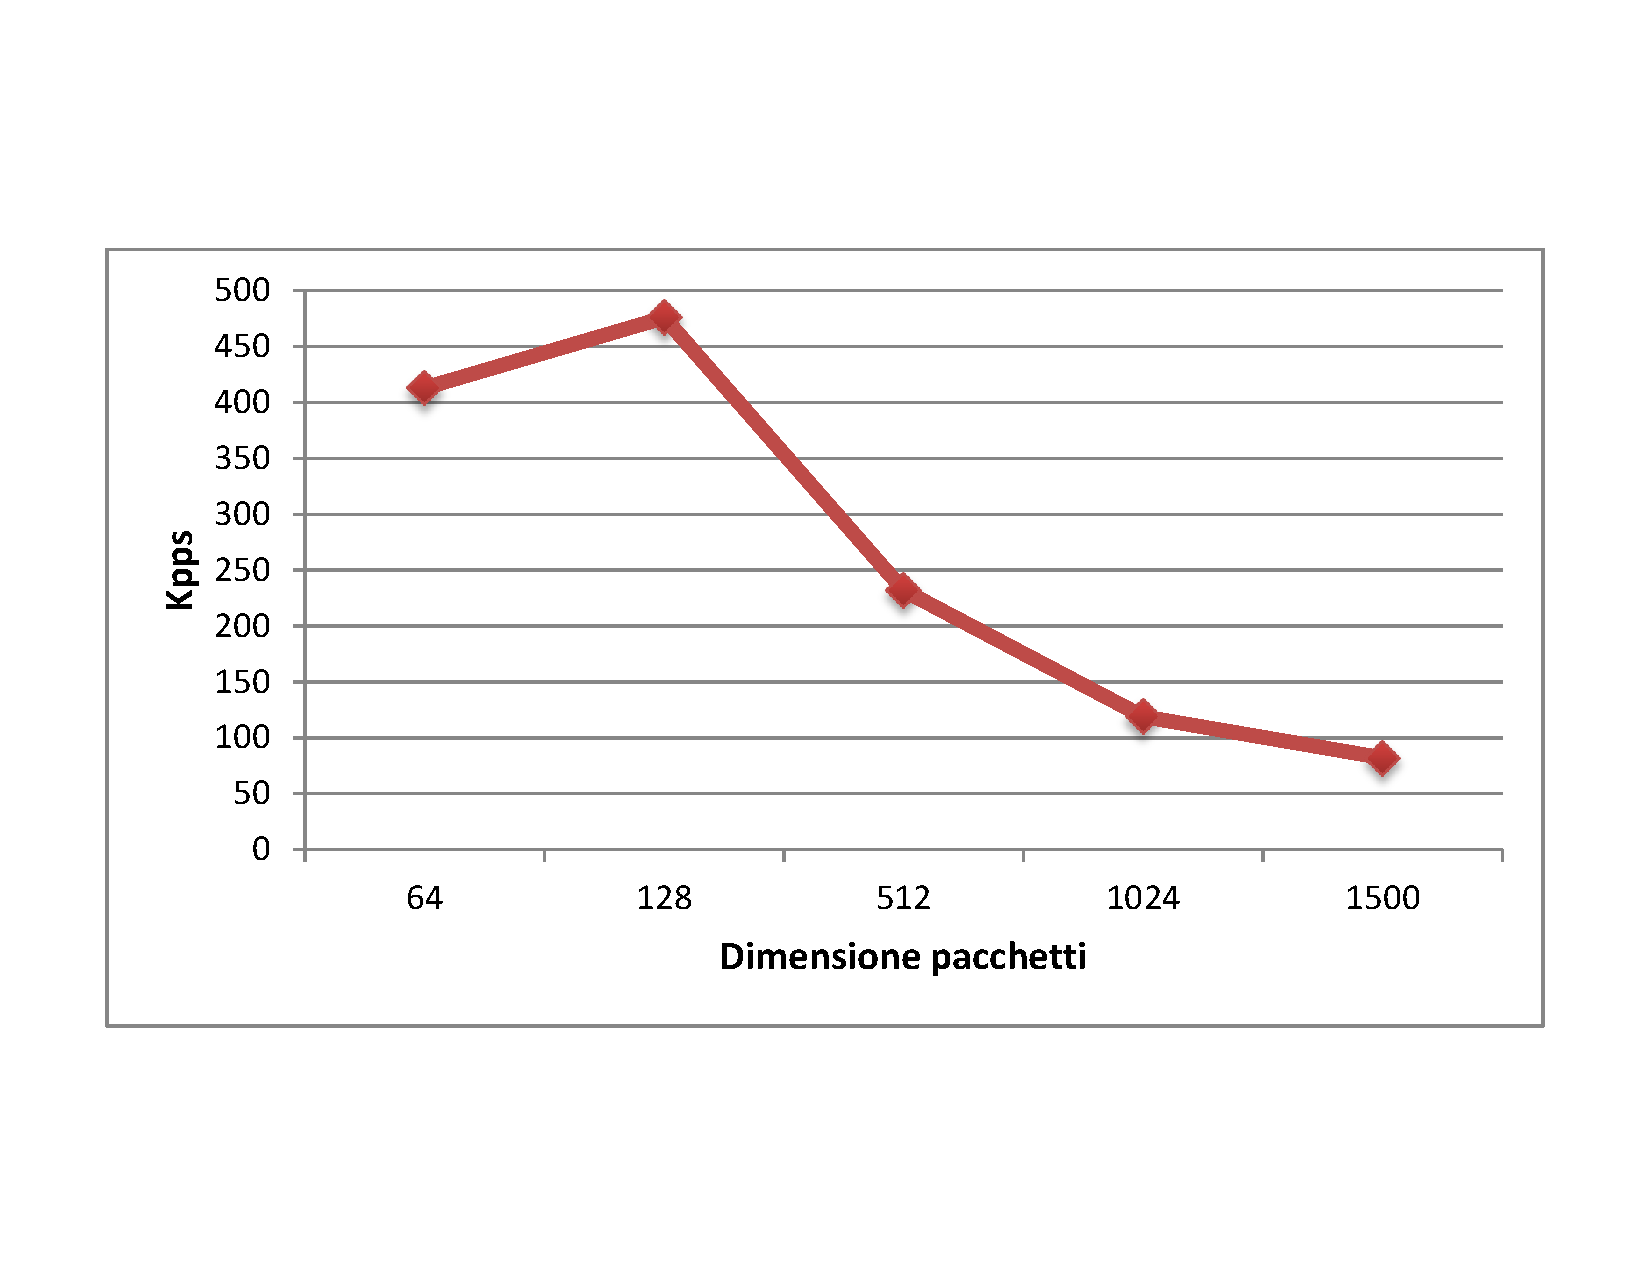
\includegraphics[scale=0.5]{img/kpps.pdf}
\caption{Capacità elaborativa di 4 thread \emph{monitor}}\label{kpps}
\end{center}
\end{figure}

\clearpage
A questo punto, per valutare il numero contemporaneo di sessioni tracciabili al secondo, si è usato un indice massimo di perdita di eventuali informazioni relativamente ad esse, aumentandole via via. Mantenendo il rate trasmissivo ancora a 1 Gbps, 4 thread \emph{monitor}, e la dimensione dei pacchetti a 512 byte, si sono ottenuti risultati davvero ottimi, mostrati nel grafico \ref{sess} seguente.

\begin{figure}[H] % htbp
\begin{center}
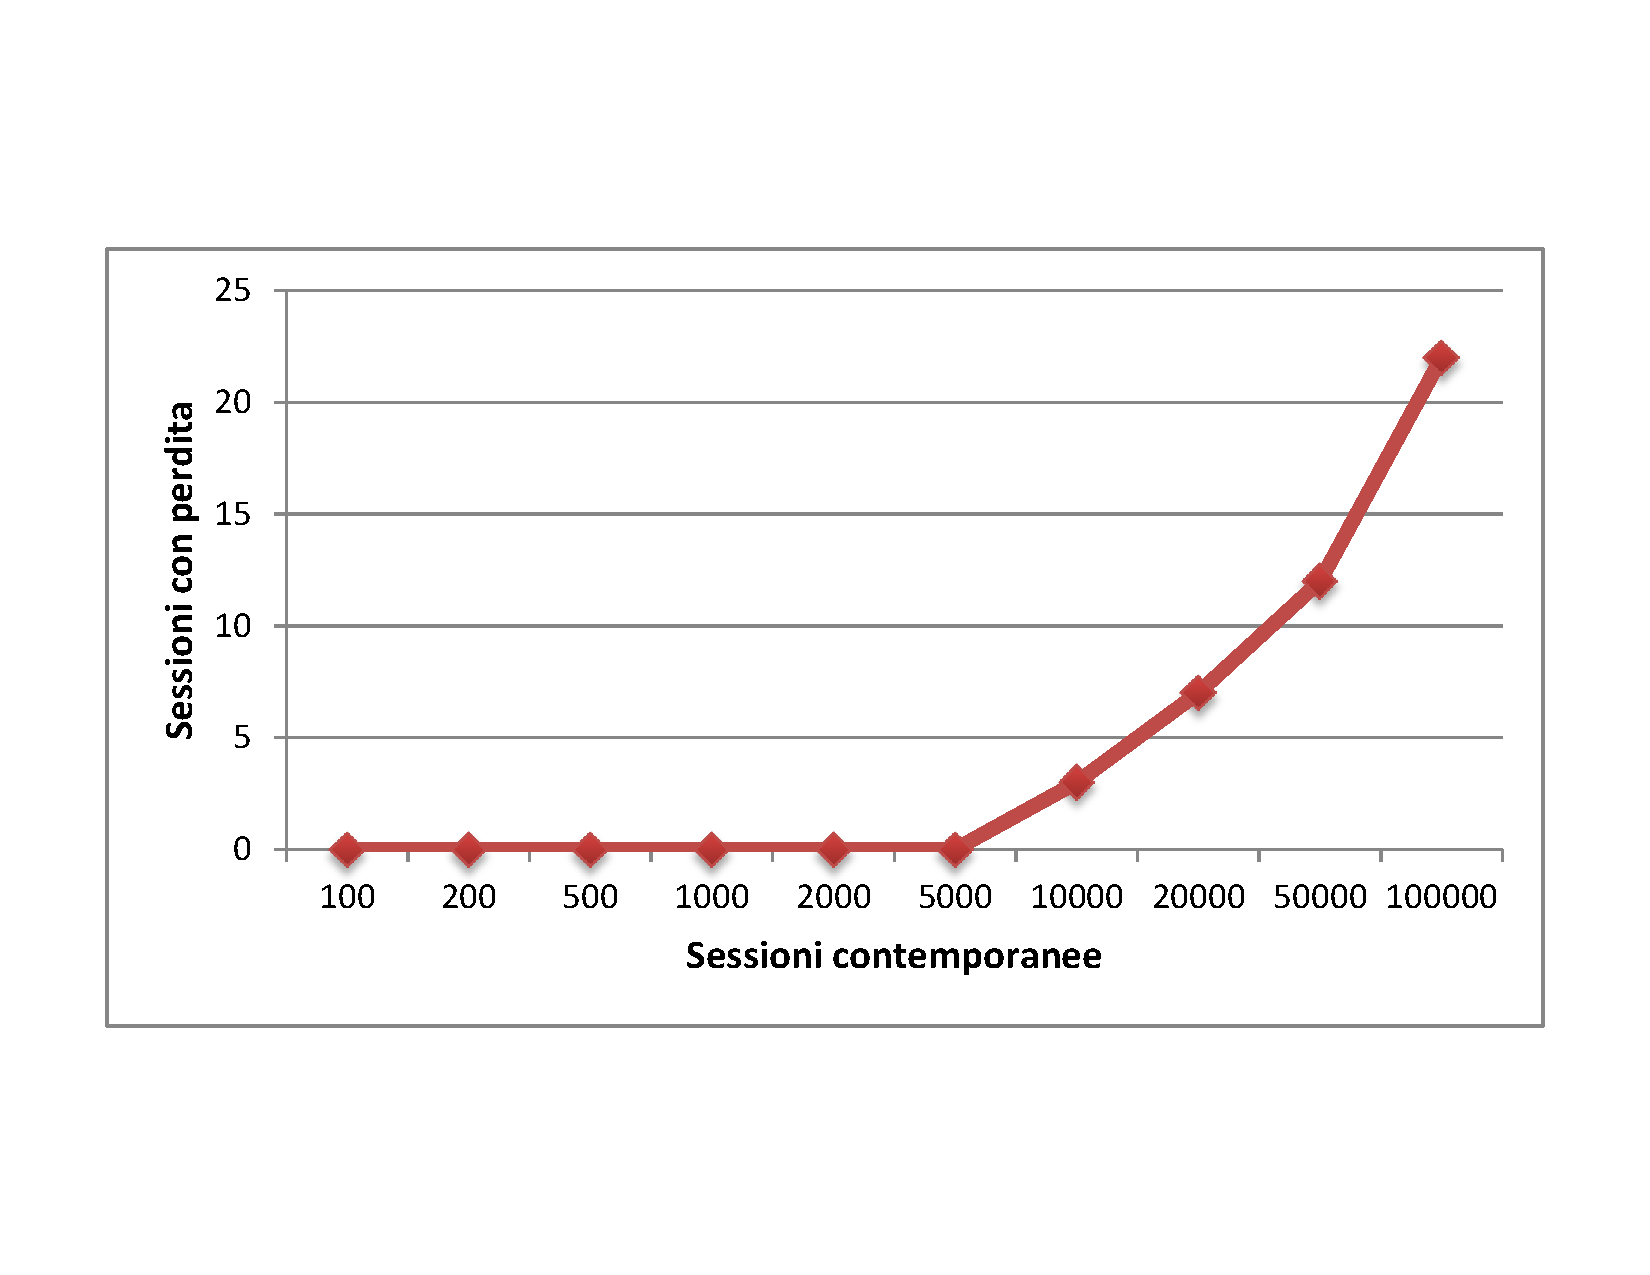
\includegraphics[scale=0.5]{img/sess.pdf}
\caption{Perdite su sessioni contemporanee}\label{sess}
\end{center}
\end{figure}

\clearpage
L'ultimo e più importante aspetto considerato, è stato quello del numero di migliaia di pacchetti processabili all'aumentare dei thread \emph{monitor} utilizzati. Questo è stato effettuato iniettando traffico reale limitato alla dimensione di 512 byte il pacchetto. I risultati, davvero ottimi, sono sintetizzati nel seguente grafico \ref{perf}.

\begin{figure}[H]
\begin{center}
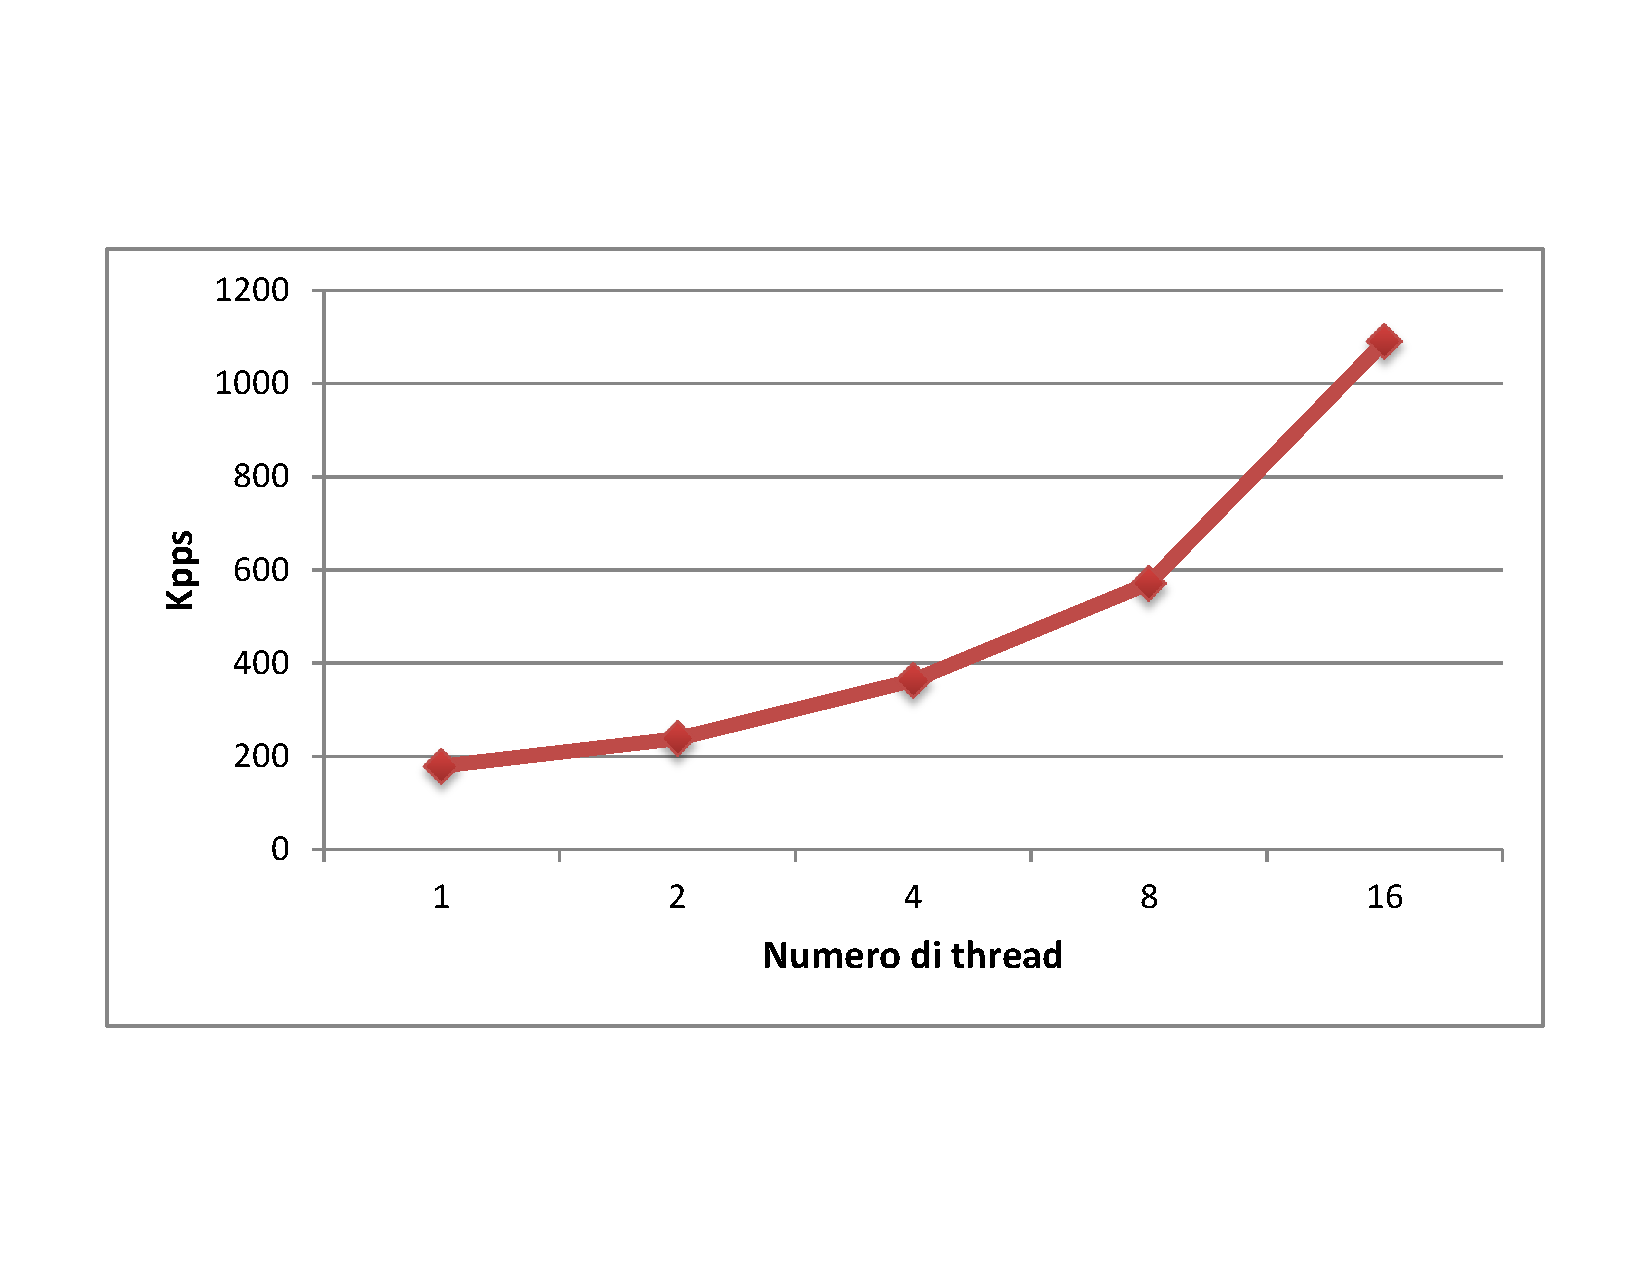
\includegraphics[scale=0.5]{img/perf.pdf}
\caption{Performance reali dell'applicazione}\label{perf}
\end{center}
\end{figure}

I risultati dei vari test sono dunque incoraggianti per lo sviluppo futuro e perfettamente in linea, se non superiori, con gli obiettivi prestabiliti.

Si ritiene comunque utile e doveroso eseguire test approfonditi sul software anche in base ai criteri stabiliti dalla RFC 3511 \cite{rfc3511}, riguardante la \emph{Metodologia di Benchmarking per le Performance dei Firewall}, al fine di ottenere dei dati oggettivi e standardizzati per una futura versione di rilascio.